\chapter[Referencial Teórico]{Referencial Teórico}

\section{Potenciais Evocados Visuais}

Seres humanos, entre outras espécies de animais \cite{Rager1998}, quando confrontados com luzes de amplitude oscilatória em seu campo de visão apresentam em seu cérebro atividades elétricas oscilatórias de mesma frequência que a do estímulo \cite{Regan1986} através de caminhos neurais. As tensões criadas por esses mecanismos cerebrais, orquestrados pelo sistema nervoso visual, quando associadas a algum evento visual como mudanças rápidas na luz, variações de frequência constante na luminosidade, até mesmo oscilações espaciais, como um disco xadrez girando \cite{hanHighlyInteractiveBrain2018} - vide Figura \autoref{fig: fig1}$C_6$ -, são chamadas de \textit{Potenciais Evocados Visuais} (VEPs), que podem ser contrapostos aos Potenciais Evocados (EPs) Espontâneos, que são atividades cerebrais alheias ao estímulo visual realizado a fim de elicitar essa resposta.

Entre os vários estudos sobre VEPs, podemos fundamentalmente dividi-los em duas formas de análise: os que utilizam a fase transiente do sinal elétrico gerado, os VEPs \textit{Transientes}, ou os que fazem uso do estado permanente do sinal elétrico, os VEPs de \textit{Estado Permanente} (SSVEPs) \cite{Regan1982}. Ao realizar um estímulo visual em uma pessoa, enquanto capta seus sinais cerebrais através de um eletroencefalograma (EEG) com eletrodos em seu escalpo, os VEPs Transientes irão surgir em um momento inicial e, caso o estímulo continue sendo executado e visualizado, eles irão se transformar em SSVEPs de forma paulatina. Pelo fato de o sistema visual, assim como o auditivo - que também pode gerar potenciais evocados \cite{John2000} -, apresentar um comportamento não-linear, esses dois tipos de VEPs podem trazer informações complementares sobre o sistema visual e a geração de seus impulsos elétricos \cite{Regan1982}. 

Como dito anteriormente de forma breve, há diferentes formas de se elicitar VEPs \cite{odom2004, Vialatte2010}, veja a Figura \autoref{fig: fig1}. As mais usuais são:  

\begin{itemize}
    \item Por flashes: aqui, uma fonte de luz é acesa e apagada constantemente. Podem ser criados através de telas de computador (com um quadrado de cor única sendo ligado e desligado), diodos de emissão de luz (LEDs), entre outros (veja \autoref{fig: fig1}A,B e $C_1$)

    \item Reversão de padrão: aqui, estímulos no formato de tabuleiros de xadrez, ou em uma sequência de listras, têm suas cores alternadas de forma constante. Geralmente são padrões em branco e preto;
    
    \item Padrão ON/OFF: novamente temos os padrões citados acima, porém nessa forma de estímulo os retângulos (ou listras) são constantemente ligados e desligados. Ou seja, em um padrão de xadrez branco e preto, os retângulos brancos iriam se tornar pretos e então novamente brancos, de forma contínua e repetitiva.
\end{itemize}

\begin{figure}[ht]
    \caption{Exemplos de estímulos utilizados para evocar VEPs.}
    \label{fig: fig1}
    \centering
    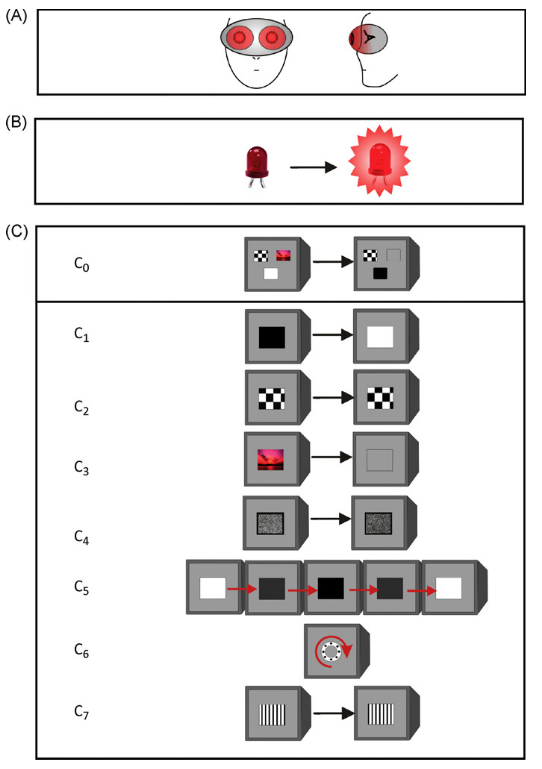
\includegraphics[width=0.7\textwidth]{stimuli.png}
    \legend{"Steady-state visually evoked potentials: Focus on essential paradigms and future perspectives" por F.B. Vialatte \textit{et al.}, 2010, Progress in Neurobiology, v. 90, n.4, p. 420. Copyright 2009 Elsevier Ltd}
\end{figure}

Em 1966 foi feito um estudo a fim de extrair informações dos sinais, tanto de VEPs transientes quanto de SSVEPs, através de flashes de uma lâmpada xenon \cite{Regan1966}. Tal estudo trouxe à época importantes informações sobre a obtenção de VEPs elicitados por flashes monocromáticos modulados por ondas senoidais, enquanto que um computador analógico realizava medições e extrações de qualquer EP que sempre mantivesse uma fase constante em relação ao estímulo. Pode-se então notar que uma das características que podem fornecer informações sobre um SSVEP é a fase \cite{Kluge2007,Liang2020}. Porém, focaremos em outras características desses potenciais que serão alvo do estudo.

\section{Potenciais Evocados Visuais de Estado Permanente (SSVEPs)}\label{ssvep}

Como dito anteriormente, SSVEPs são sinais elétricos gerados no cérebro durante um estímulo visual oscilatório de frequência constante. Portanto, apesar de quando imediatamente colhido o sinal seja uma função da tensão (geralmente em $\mu V$) em relação ao tempo, em vários trabalhos temos o uso de transformadas desses sinais para o domínio espectral. Talvez seja interessante uma definição com maior exatidão: "SSVEPs are evoked responses induced by flickering visual stimuli. SSVEPs are periodic, with a stationary distinct spectrum showing characteristic SSVEPs peaks, stable over time" ~\cite{Vialatte2010}. Todavia, é ainda indefinido quais são as frequências limítrofes capazes de gerar tais respostas. 

Em um primeiro momento, Regan \cite{Regan1982} apresentou um modelo de como se comportaria a amplitude de tais respostas em domínio espectral trouxe a análise para frequências entre, aproximadamente, 5 e 55 Hz. A média das amplitudes das componentes de frequência da resposta de SSVEP de mesma frequência que o estímulo pode ser vista na Figura \autoref{fig: fig2}. Podemos ver claramente três picos de amplitude ao redor de 10, 16 e 50 Hz. Em um estudo um pouco mais recente, Wang \cite{Wang2006} fez uso de praticamente o mesmo limite de frequências, de 5 a 45 Hz; encontrando picos centrados ao redor das frequências de 15, 31 e 41 Hz e afirmando que essas três regiões são comumente chamadas de regiões de baixa-, média- e alta-frequência.

\begin{figure}[ht]
    \caption{Comportamento da média de potenciais evocados elicitados por uma luz oscilando a uma frequência F.}
    \label{fig: fig2}
    \centering
    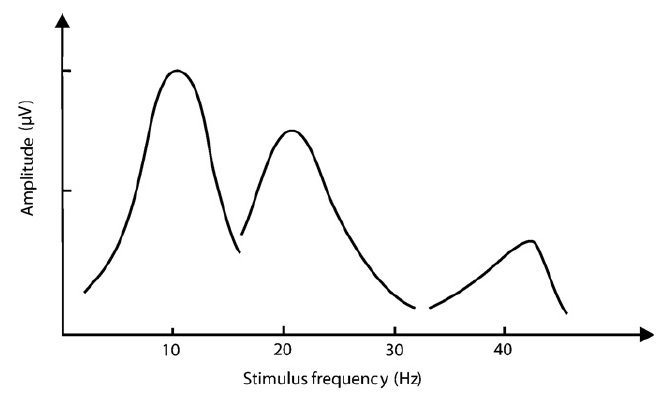
\includegraphics[width=0.7\textwidth]{frequency_peaks.png}
    \legend{"Comparison of Transient and Steady-state Methods" por D. Regan, 1982, Annals of the New York Academy of Science, v. 388, n.1, p. 48}
\end{figure}

Entretanto, estudos recentes fazem uso de um maior espectro, tendo em vista que há evidências de comportamento responsivo, ressonante, a frequências ultrapassando o limite de percepção consciente ,também chamado de \textit{critical flicker-fusion frequency} (CFF), alcançando frequências em torno de 90 Hz \cite{Pastor2003, Herrmann2001, RamosJunior2011}. A CFF pode ser explicada como o valor de frequência em que seres humanos passam a enxergar flashes oscilatórios como luzes contínuas, não-oscilatórias. Além disso, também é possível encontrar harmônicas superiores das frequências de estimulação nos sinais de SSVEPs \cite{Muller2005a}.

\section{Aplicabilidades e Empecilhos}

Hoje, vários estudos já encontraram diversas aplicações utilizando extração de dados de sinais de SSVEPs. Algumas delas são: análise de atenção visual \cite{Muller2006}; análise de distrações intermodais \cite{Heim2019}; auxílio no diagnóstico de autismo \cite{Belmonte2000}; e, talvez a que seja mais amplamente estudada, a utilização de SSVEPs para interfaces cérebro-computador (BCIs) a fim de enviar comandos sem a necessidade de movimento muscular \cite{Wang2006, Sakurada2015, Wang2017}.

Contudo, além da frequência do estímulo por si só, outros fatores também interferem com a amplitude das respostas de SSVEPs. Entre eles: o espaçamento entre as listras/grades em um estímulo realizado por um padrão \cite{Regan1978}, chamado de frequência espacial; a porcentagem de contraste aplicado nas oscilações \cite{Regan1978}, da luminosidade ou da cor do estímulo; a cor do estímulo \cite{GodinezTello2015, Parra2007}; a fadiga do usuário, tanto visual quanto de cansaço por si só \cite{Zhang2019, Chang2014}; entre outros.